\documentclass[12pt]{article}
\usepackage[a4paper,margin=2.5cm]{geometry}
\usepackage{amsmath, amssymb, amsthm}
\usepackage{bm}
\usepackage{hyperref}
\usepackage{graphicx}
\usepackage{caption}
\usepackage{listings}
\usepackage{xcolor}
\usepackage{float}
\usepackage{placeins}
\graphicspath{{figures/}}

% Code style
\lstdefinestyle{code}{
  basicstyle=\ttfamily\small,
  numbers=left,
  numberstyle=\tiny,
  numbersep=8pt,
  keywordstyle=\color{blue},
  commentstyle=\color{teal!70!black},
  stringstyle=\color{orange!70!black},
  showstringspaces=false,
  breaklines=true,
  frame=single,
  framerule=0.3pt,
  rulecolor=\color{black!15}
}
\lstset{style=code}

\title{Comprehensive Guide to Convolutional Neural Networks}
\author{}
\date{\today}

\begin{document}
\maketitle

\section{CNN Structure and Operating Principles}
Convolutional neural networks (CNNs) exploit spatial locality and translation invariance by sharing weights across spatial positions. An input image tensor $\mathbf{X} \in \mathbb{R}^{C_{\mathrm{in}} \times H \times W}$ is convolved with kernels $\mathbf{K} \in \mathbb{R}^{C_{\mathrm{out}} \times C_{\mathrm{in}} \times k_h \times k_w}$ to produce feature maps:
\begin{equation}
  Y_{c,i,j} = \sum_{c'=1}^{C_{\mathrm{in}}} \sum_{u=0}^{k_h-1} \sum_{v=0}^{k_w-1} K_{c,c',u,v} \; X_{c',\, i s + u - p,\, j s + v - p},
\end{equation}
where $s$ is the stride and $p$ the padding. Stride controls downsampling, while padding preserves boundary information. Figure~\ref{fig:cnn_structure} illustrates how receptive fields grow across layers.

\subsection{Feature Hierarchies}
Early convolutional layers learn edge and texture detectors; middle layers capture motifs such as corners or object parts; deeper layers integrate global semantics. Weight sharing dramatically reduces parameter counts compared with fully connected layers.

\subsection{Padding, Stride, and Dilation}
Padding extends the input with zeros (or reflection/replication) so that convolutions can cover border pixels. Dilation introduces gaps between kernel elements, expanding the receptive field to $\mathit{RF} = (k - 1) d + 1$ without increasing parameters. Careful combinations of stride and dilation maintain resolution while encoding global context.

\subsection{Pooling and Downsampling}
Pooling layers summarize local neighborhoods, providing robustness to small translations. Max pooling emphasizes the strongest activation, average pooling smooths representations, and strided convolutions can replace pooling entirely for learnable downsampling. Global average pooling reduces each feature map to a scalar, enabling fully convolutional classifiers.

\subsection{Normalization and Activation}
CNNs typically use rectified linear unit (ReLU) or its variants (LeakyReLU, GELU) to introduce nonlinearity. Batch normalization normalizes activations using mini-batch statistics, mitigating internal covariate shift and enabling higher learning rates. Layer normalization or group normalization are alternative choices for small batches.

\begin{lstlisting}[language=Python, caption={PyTorch implementation of a convolutional stem with normalization and pooling.}]
import torch.nn as nn

class ConvStem(nn.Module):
    def __init__(self, in_channels=3, hidden_channels=(64, 128, 256)):
        super().__init__()
        layers = []
        current = in_channels
        for out_channels in hidden_channels:
            layers += [
                nn.Conv2d(current, out_channels, kernel_size=3, stride=1, padding=1, bias=False),
                nn.BatchNorm2d(out_channels),
                nn.ReLU(inplace=True),
                nn.MaxPool2d(kernel_size=2, stride=2)
            ]
            current = out_channels
        self.stem = nn.Sequential(*layers)

    def forward(self, x):
        return self.stem(x)
\end{lstlisting}

\begin{figure}[H]
  \centering
  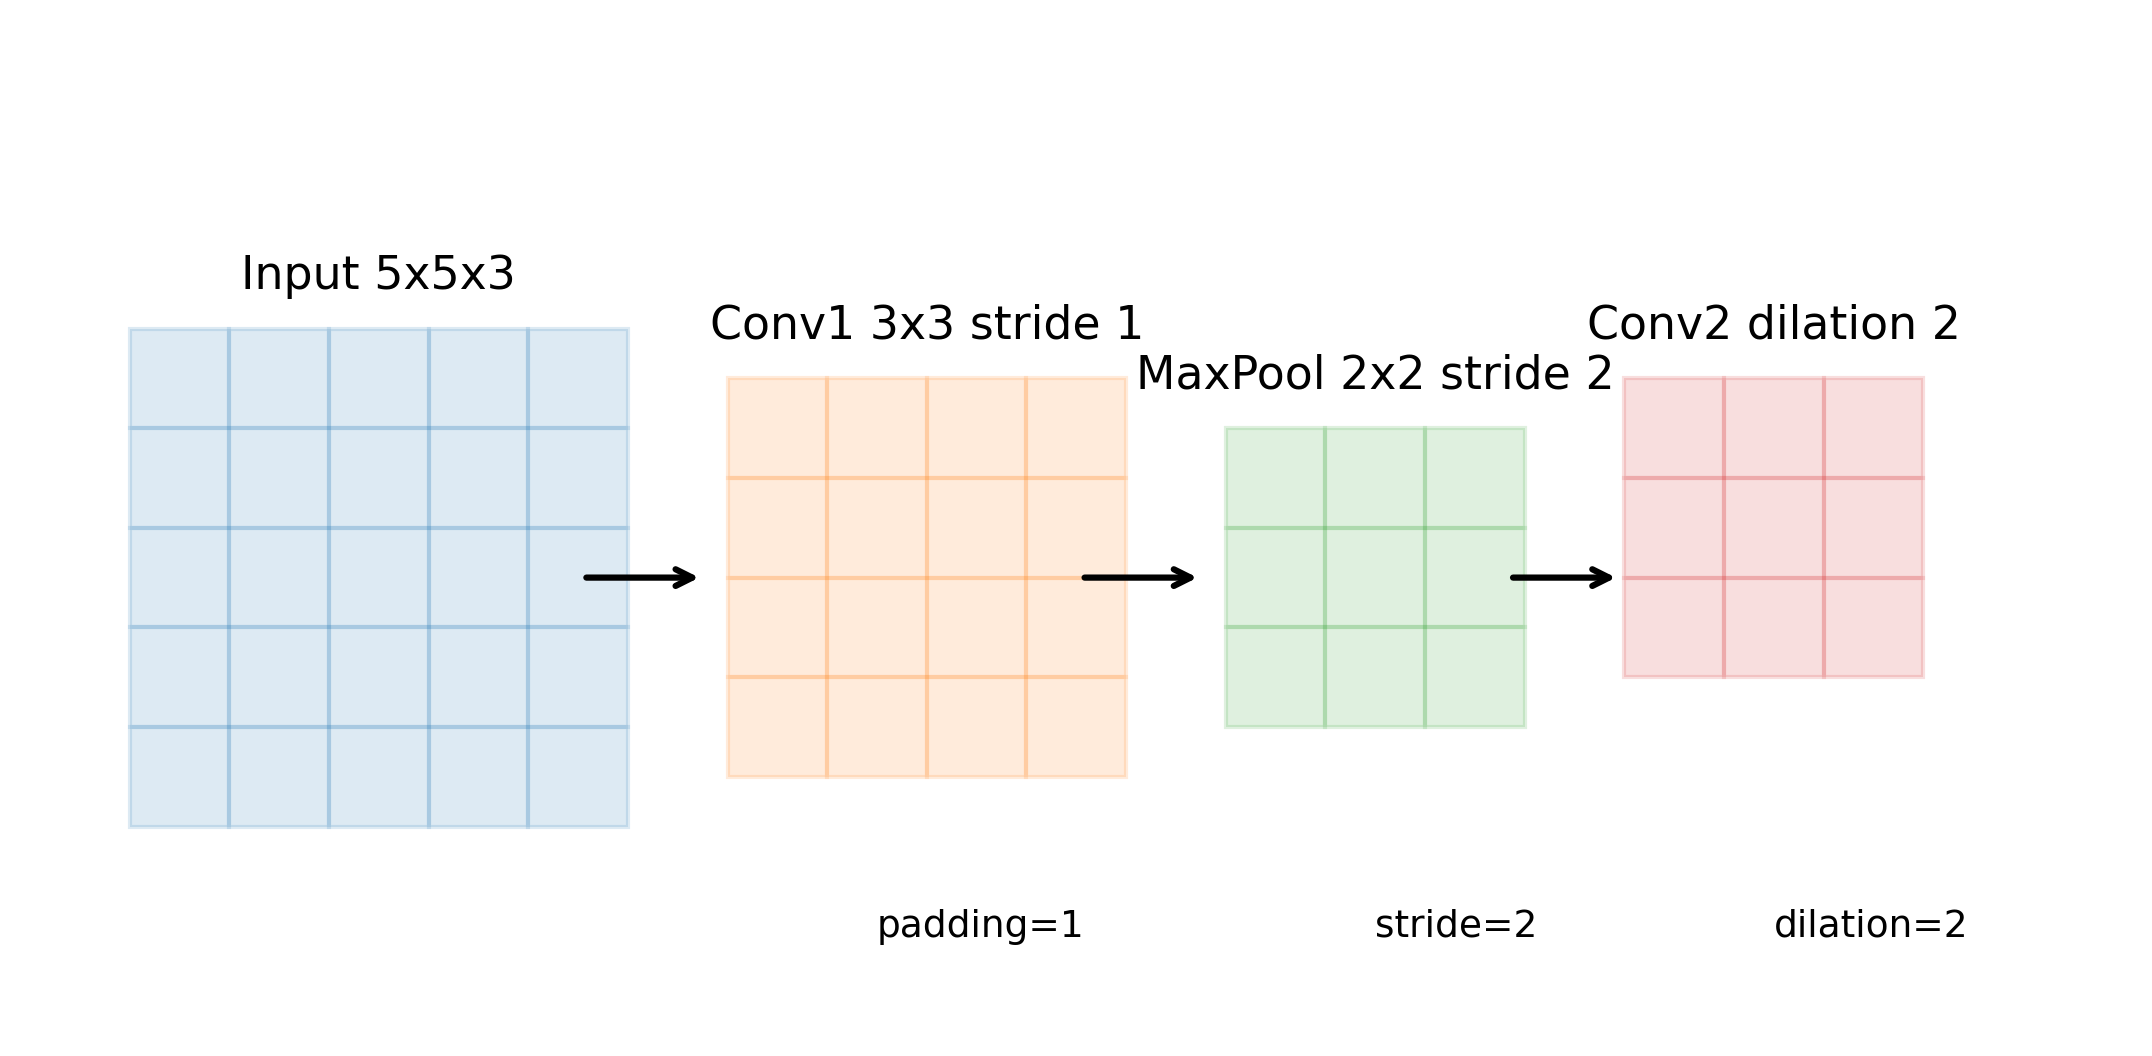
\includegraphics[width=0.85\linewidth]{cnn_structure_receptive_field.png}
  \caption{Illustration of convolutions, padding, stride, and pooling expanding receptive fields across layers.}
  \label{fig:cnn_structure}
\end{figure}
\FloatBarrier

\section{Classical Architectures: A Comparative Overview}
Over three decades, CNN architectures evolved to address optimization challenges, computational efficiency, and scalability. Figure~\ref{fig:cnn_timeline} highlights key milestones, and Table~\ref{tab:cnn_compare} contrasts design choices.

\subsection{LeNet-5 (1998)}
Yann LeCun's LeNet pioneered digit recognition by stacking convolution and subsampling layers before fully connected classifiers. Its use of weight sharing enabled practical training on limited hardware.

\subsection{AlexNet (2012)}
AlexNet conquered ImageNet using deeper networks, ReLU activations to avoid saturation, extensive data augmentation, and dropout regularization. Two GPUs processed disjoint halves of feature maps, showcasing the importance of hardware acceleration.

\subsection{VGG (2014)}
VGG-16/19 advocated uniform $3 \times 3$ convolutions stacked deep, demonstrating that depth and small kernels can approximate larger receptive fields with fewer parameters. The model's simplicity made it a go-to backbone for transfer learning.

\subsection{ResNet (2015)}
Residual connections allowed ResNet to train over 150 layers by reformulating layers as residual functions $\mathcal{F}(\mathbf{x}) + \mathbf{x}$. Identity shortcuts preserve gradient flow and enable easier optimization.

\subsection{Inception Family (2014--2016)}
GoogLeNet (Inception-v1) introduced multi-branch modules combining various kernel sizes. Later versions factorized $5 \times 5$ into stacked $3 \times 3$ convolutions and added batch normalization. Inception-v3/v4 further refined factorization and regularization.

\subsection{EfficientNet (2019)}
EfficientNet scales depth, width, and resolution via a compound coefficient, starting from a mobile inverted bottleneck block with squeeze-and-excitation attention. Balanced scaling achieved state-of-the-art accuracy with fewer FLOPs.

\begin{table}[H]
  \centering
  \caption{Comparison of influential CNN architectures. Parameter counts and FLOPs are approximate for ImageNet-scale models.}
  \label{tab:cnn_compare}
  \begin{tabular}{lccccl}
    \hline
    Architecture & Year & Depth & Params (M) & FLOPs (G) & Signature features \\
    \hline
    LeNet-5 & 1998 & 7 & 0.06 & 0.002 & Conv + subsampling for digits \\
    AlexNet & 2012 & 8 & 61 & 1.5 & ReLU, dropout, large kernels \\
    VGG-16 & 2014 & 16 & 138 & 15.5 & Stacked $3\times3$ convs \\
    ResNet-50 & 2015 & 50 & 25 & 4.1 & Residual bottlenecks \\
    Inception-v3 & 2016 & 48 & 24 & 5.7 & Multi-branch factorized convs \\
    EfficientNet-B4 & 2019 & 82 & 19 & 4.2 & Compound scaling, MBConv \\
    \hline
  \end{tabular}
\end{table}

\begin{figure}[H]
  \centering
  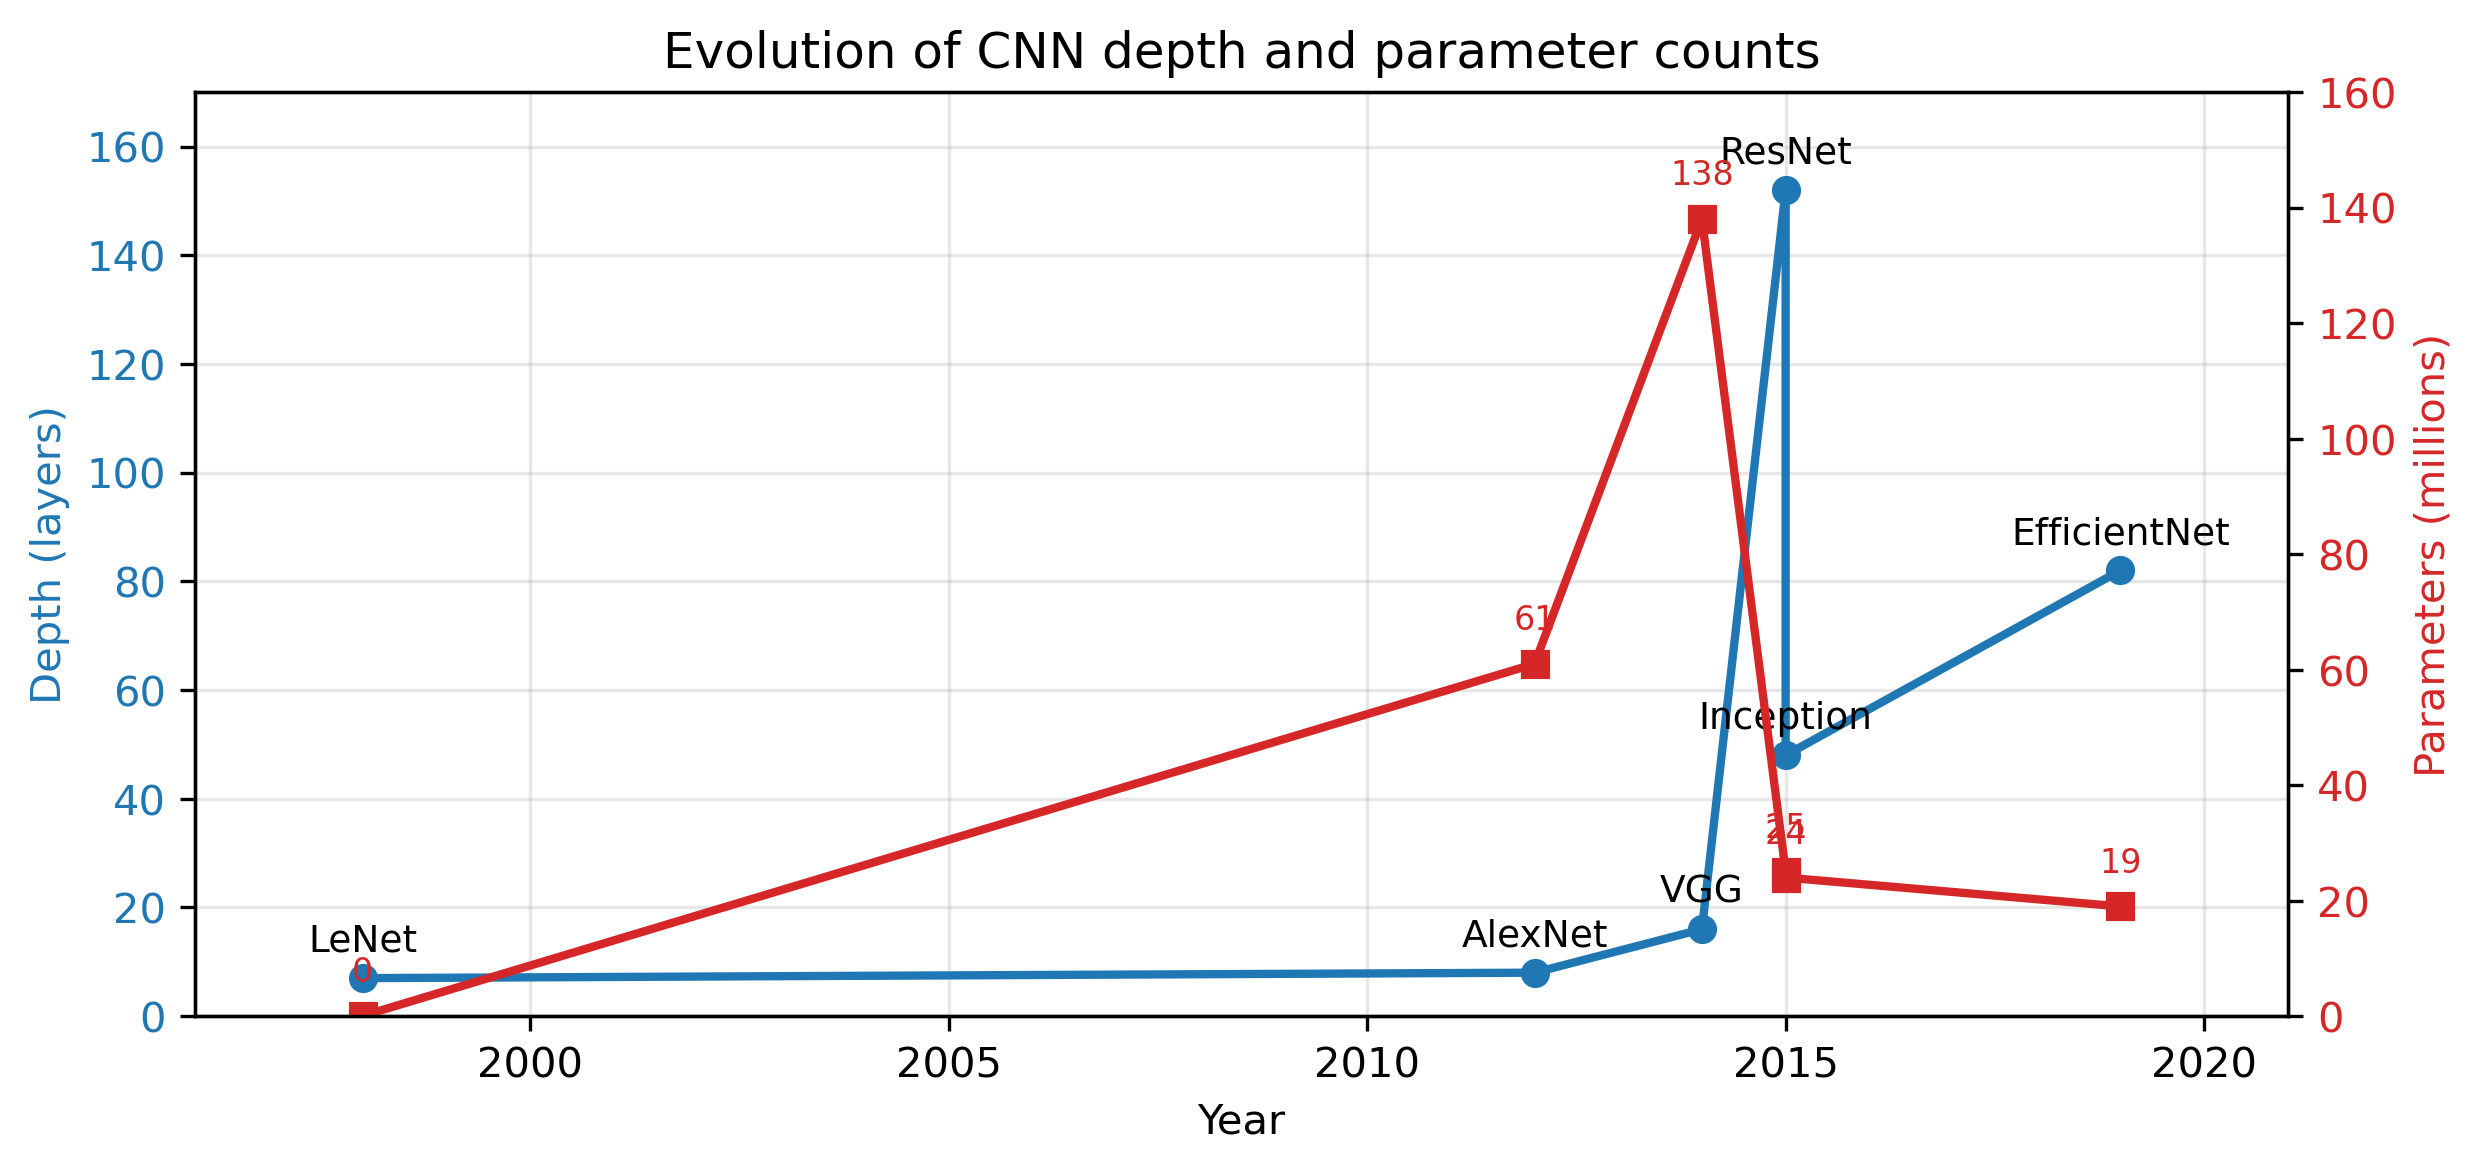
\includegraphics[width=0.85\linewidth]{cnn_architecture_evolution.png}
  \caption{Timeline of CNN breakthroughs and their core innovations.}
  \label{fig:cnn_timeline}
\end{figure}
\FloatBarrier

\section{Applications Across Vision Tasks}
CNNs underpin diverse computer vision applications. Figure~\ref{fig:cnn_applications} sketches high-level pipelines.

\subsection{Image Classification}
Classification networks map an input image to class probabilities. Modern classifiers leverage pretrained backbones, global pooling, and label smoothing to combat overconfidence. Mixup and CutMix augmentation further regularize training.

\subsection{Object Detection}
Detection augments CNN backbones with localization heads. Two-stage detectors (Faster R-CNN) generate region proposals before refinement, while one-stage models (YOLOv8, RetinaNet) predict boxes and classes densely. Feature pyramid networks (FPN) reuse multi-scale feature maps to detect objects spanning wide size ranges.

\subsection{Semantic Segmentation}
Segmentation assigns labels to individual pixels. Encoder-decoder architectures (U-Net, SegNet) recover spatial detail via skip connections. Dilated convolutions (DeepLab), pyramid pooling modules (PSPNet), and attention enhance context reasoning. Metrics such as mean Intersection-over-Union (mIoU) measure performance.

\subsection{Beyond 2D Vision}
CNNs extend to video (3D convolutions, TimeSformer hybrids), medical imaging (multi-scale U-Nets), and multimodal perception (CNN backbones fused with transformers). Lightweight variants (MobileNet, ShuffleNet) enable deployment on edge devices.

\begin{figure}[H]
  \centering
  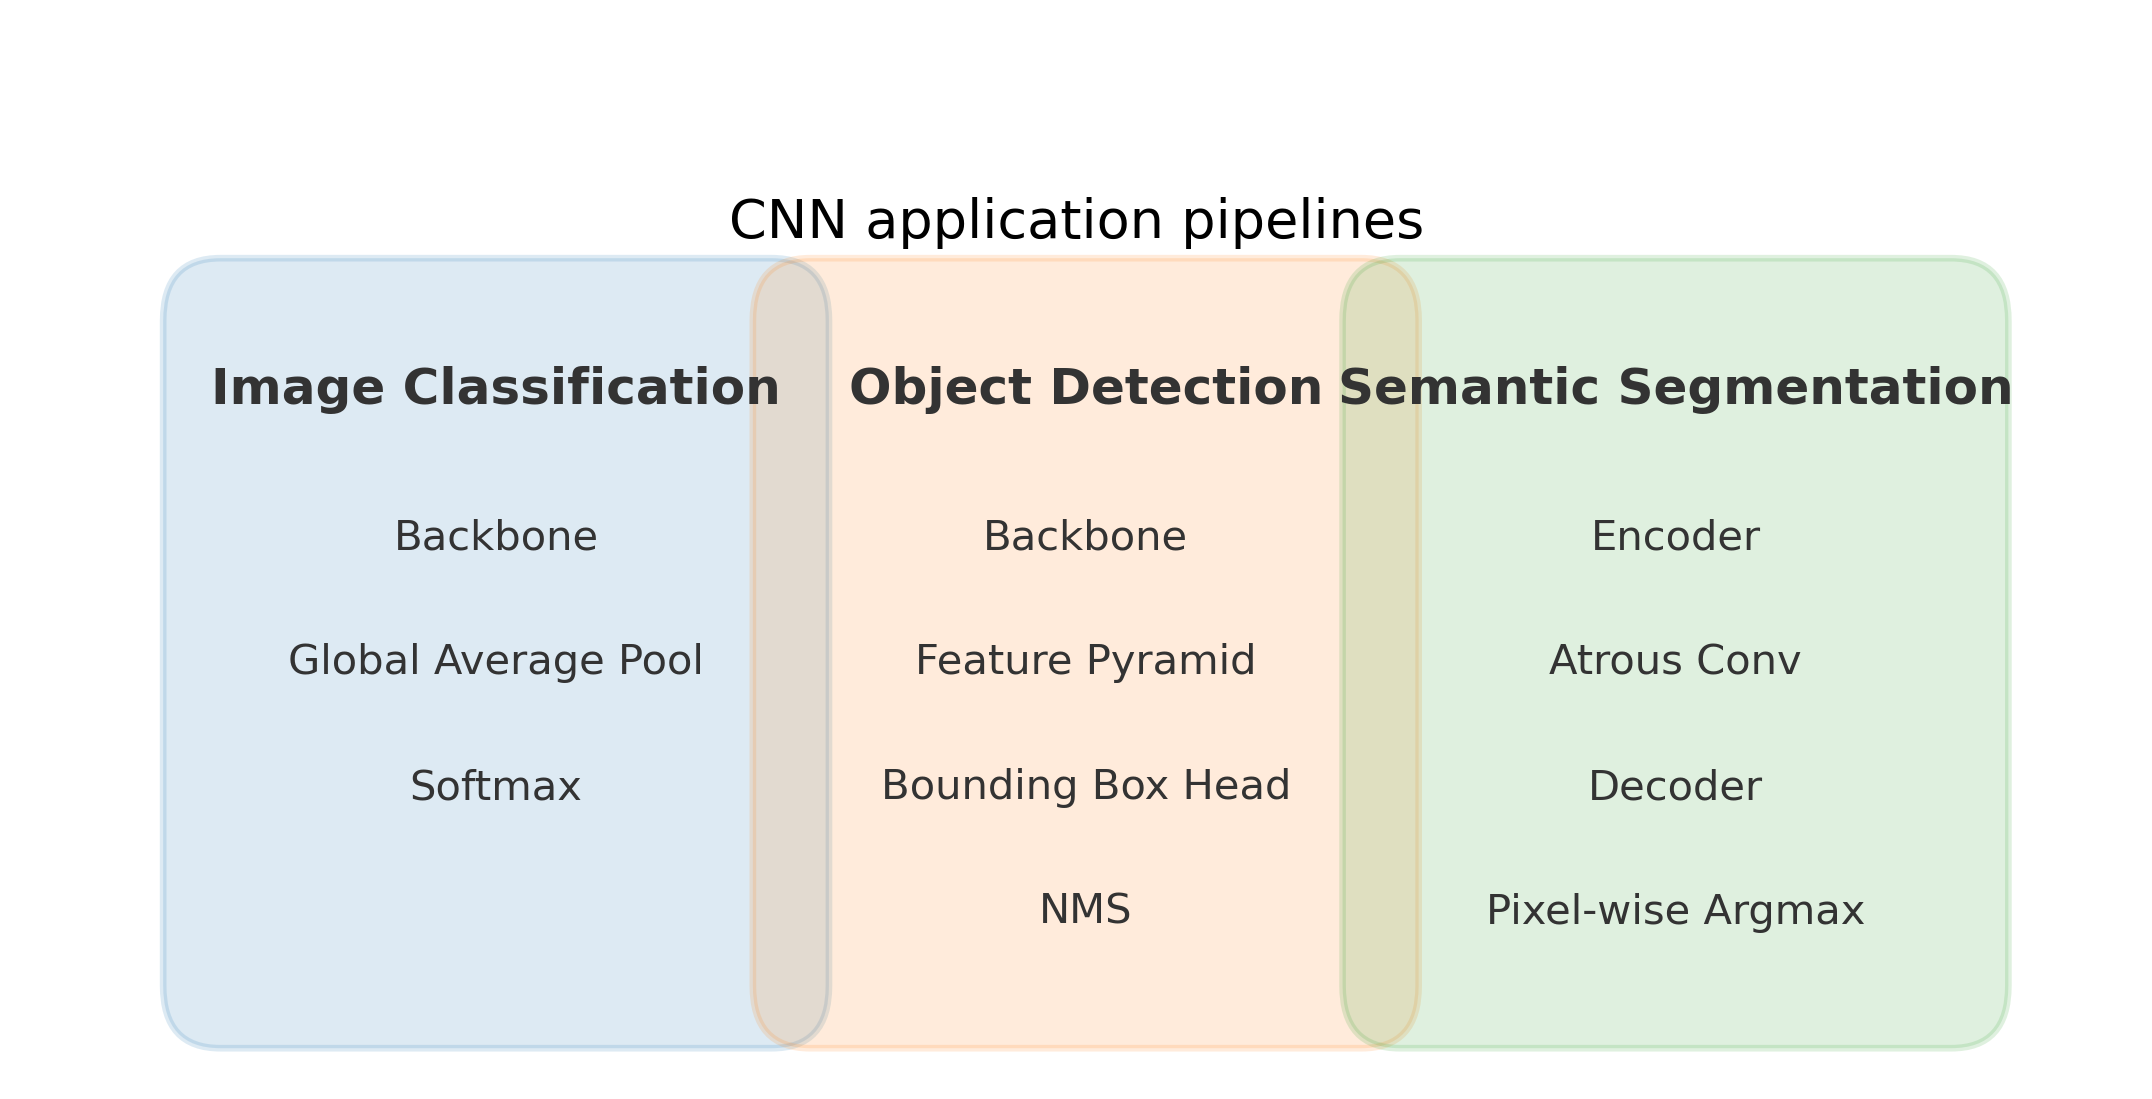
\includegraphics[width=0.85\linewidth]{cnn_applications_overview.png}
  \caption{Representative CNN application pipelines: classification, detection, and semantic segmentation.}
  \label{fig:cnn_applications}
\end{figure}
\FloatBarrier

\section{Training and Deployment Tips}
\begin{itemize}
  \item \textbf{Initialization \\& normalization:} Use He initialization with BatchNorm or GroupNorm for stable gradients.\item \textbf{Regularization:} Apply augmentation (random crop, color jitter, CutMix), dropout, and stochastic depth to combat overfitting.\item \textbf{Optimization:} Cosine learning-rate schedules with warmup and momentum SGD remain strong baselines; adaptive optimizers aid rapid prototyping.\item \textbf{Efficiency:} Prune filters, quantize weights, or use depthwise separable convolutions for mobile deployment.\item \textbf{Monitoring:} Track task-specific metrics (Top-1 accuracy, mAP, mIoU) and visualize feature maps to diagnose failures.\end{itemize}

\end{document}
